\textbf{Question: Plot $g_\gamma(x)$ vs. $x$ in the range $x\in [-{\rm FS},{\rm FS}]$ for $\gamma = 0$, $1$ and $2$. For input signals whose values are always much smaller than $\rm FS$ (in absolute value), what will be the effect of the nonlinearity?
}
\vspace{0.5cm}

\begin{figure}[H]
    \centering
    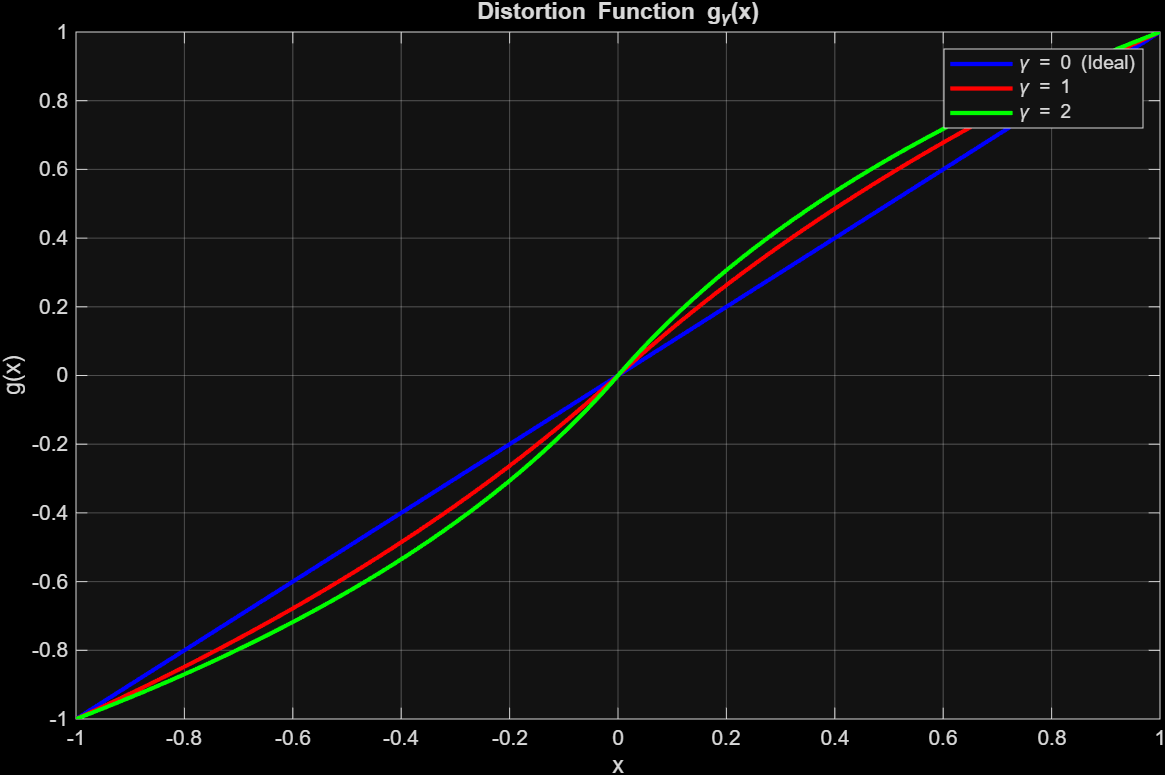
\includegraphics[width=1\textwidth]{img/task5_1.png}
    \label{fig:task5_1}
\end{figure}

\vspace{1cm}
\textbf{Question: Modify the code in {\tt quanti.m} and write a Matlab function {\tt dquanti.m} implementing this nonuniform quantizer. The format should be similar to that of {\tt quanti.m}, but including an additional input parameter {\tt gama}:}
\begin{center}
{\tt xq = dquanti( x, FS, Nbits, gama ); }
\end{center} 
\vspace{0.5cm}

We change the code as follows:
\begin{lstlisting}[language=Matlab]
    function y = dquanti(x, FS, Nbits, gama)
    if gama == 0
        g_x = x; % Si gama=0, no hay distorsion (g(x) = x)
    else
        g_x = sign(x) .* (FS / log(1 + gama)) .* log(1 + gama .* abs(x) / FS);
        g_x(x == 0) = 0;
    end

    FS    = abs(FS);
    FSbin = 2^(Nbits-1);
    LSB   = FS/FSbin;  

        y = round(g_x/LSB); 
        y = min(y, FSbin-1); 
        y = max(y, -FSbin); 
        y = y * LSB;
\end{lstlisting}

\vspace{1cm}
\textbf{Question: Generate  samples (at 100 MHz) of a full-scale sinusoid with $f_0 = 6.8359$ MHz.
Quantize them to $N=11$ bits using $\gamma = 0.003$ in {\tt dquanti}. 
Determine the SFDR in dBFS using an FFT size $M=2048$, and then with $M=512$. 
Does the SFDR depend on the FFT size? Does the noise floor depend on the FFT size? How do you explain this?
}
\vspace{0.5cm}

xd

\vspace{1cm}
\textbf{Question: Using $M=2048$, repeat the previous step for $\gamma = 0.01$ and $0.1$. Are the spectral spurs located where you would expect?
}
\vspace{0.5cm}

xd

\vspace{1cm}
\textbf{Question: Set now the amplitude to $\frac{\rm FS}{3}$. Using $M=2048$, measure the SFDR and express it in both dBFS and dBc for $\gamma=0.005$, $0.05$ and $0.1$. Will these values change if you repeat the analysis with $M=512$?
}
\vspace{0.5cm}

xd

\vspace{1cm}
\textbf{Question: Consider now samples (at 100 MHz and with 11-bit resolution) of a sinusoid with frequency $3.3202$ MHz and amplitude $\frac{\rm FS}{2}$. Obtain the THD for this nonuniform ADC with $\gamma = 0.3$ under the IEEE 1241-2000 specification, expressed in both dB and percentage.
}
\vspace{0.5cm}

xd

